\documentclass{article}

\usepackage{hyperref} 		%% for hyperlinks
\usepackage{amsmath} 		%% for align* environment
\usepackage{amsfonts} 		%% for \mathbb
\usepackage{graphicx} 	%% Include graphics
\usepackage{float} 			%% For float option H in figure environment
\usepackage{listings,lstautogobble} %% For code listings
\usepackage{xcolor}	%% For colours in code listings

%% Followinfg two lines remove the 'references' title automarically created in bibliography
\usepackage{etoolbox}
\patchcmd{\thebibliography}{\section*{\refname}}{}{}{}

%% Setup the colouring and style of code listings
\definecolor{RoyalBlue}{cmyk}{1, 0.50, 0, 0}
\lstset{language=Java,
	keywordstyle=\color{RoyalBlue},
	basicstyle=\scriptsize\ttfamily,
	commentstyle=\ttfamily\itshape\color{gray},
	stringstyle=\ttfamily,
	showstringspaces=false,
	breaklines=true,
	rulecolor=\color{black},
	autogobble=true
}

\newcommand{\R}{\ensuremath{\mathbb{R}}} %% Allows \R for real number set
\newcommand{\C}{\ensuremath{\mathbb{C}}} %% Allows \C for Complex number set

\title{Complex Grapher Documentation}
\author{William RJ Cooper}
\date{September 2018}

\begin{document}
   	\maketitle
   
   	\newpage
	\tableofcontents
	\newpage
	\section{Introduction}
		The complex grapher application sets out to visualise complex landscapes using the domain colouring method. When learning about functions, algebra, and many other topics involving real values in mathematics, most students are introduced to a graphing package. This helps them understand the functions and how they behave. It follows that similar graphing packages for complex numbers would be useful. The complex grapher sets out to achieve this as quickly, efficiently and as simply as possible. It also ships with a few extra features that make navigating the complex landscape easier.
	
		\begin{figure}[H]
			\centering
			\makebox[\linewidth]{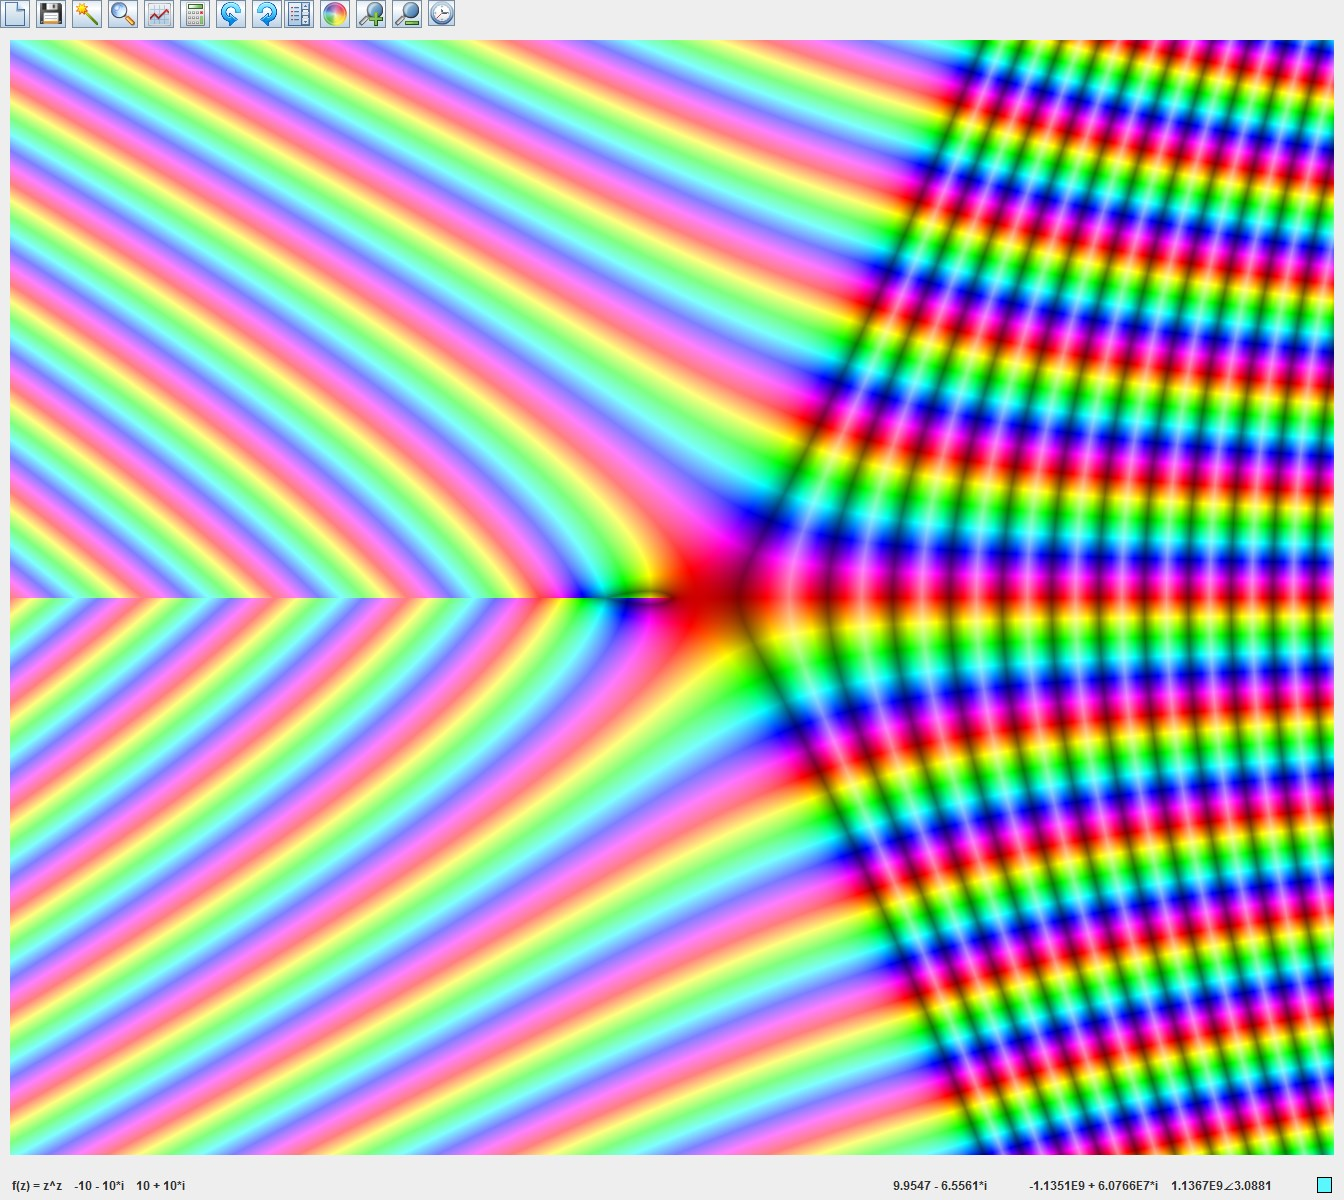
\includegraphics[scale=0.2]{z^z}}
			\textit{\caption{An image of the landscape $z^z$ with $-10-10i$ in the lower left corner, and $10+10i$ in the upper right corner.}}
			\label{graph:z^z}
		\end{figure}
	
		The user can input formulae composed of complex functions, along with coordinates for the bottom left corner, and the top left corner to display a landscape. The formula, and the two corner coordinates (referred to as minimum domain for the lower left, and maximum domain for the upper right henceforth) can all be expressed in terms of functions, operations and constants. For a comprehensive list of supported functions and constants, see the 'How to Use' section.

		\begin{figure}[H]
			\centering
			\makebox[\linewidth]{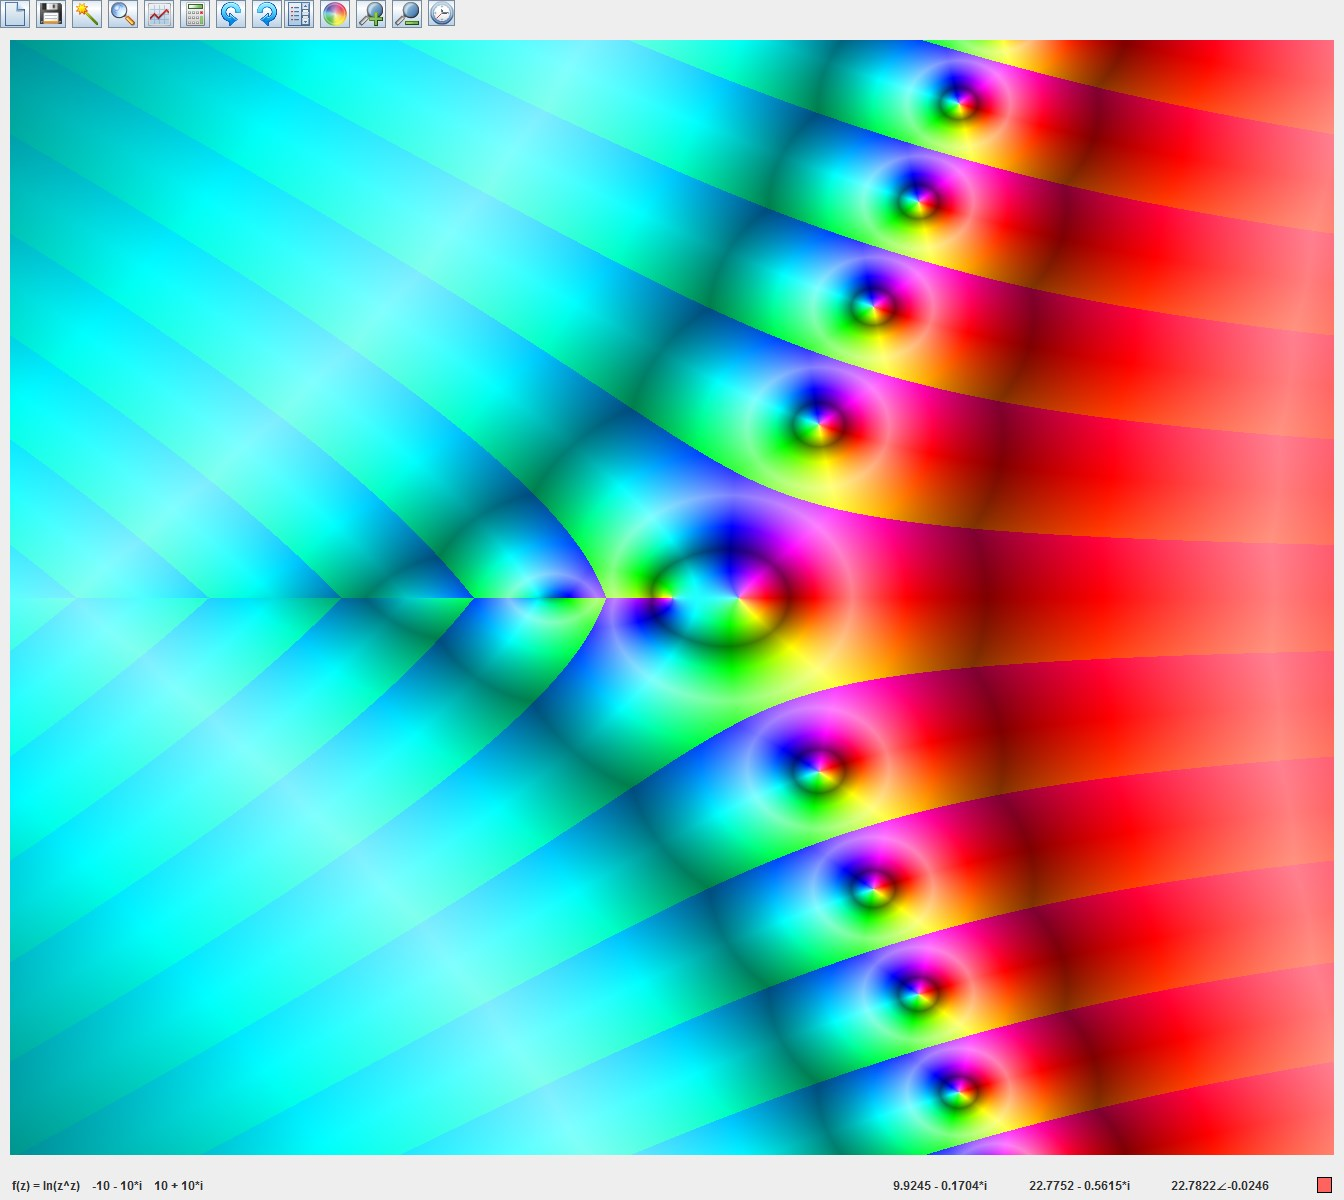
\includegraphics[scale=0.2]{ln(z^z)}}
			\textit{\caption{An image of the landscape $ln(z^z)$ with $-10-10i$ in the lower left corner, and $10+10i$ in the upper right corner.}}
			\label{graph:ln(z^z)}
		\end{figure}
	
	\section{Design features}
	
		While the Complex Grapher is not meant to be a fully complete set of complex analysis tools, it does contain a comprehensive list of features. Those features were chosen as the most popular and most useful ones. If the user requires more detailed, more specific, or more involved features, software packages like Matlab and Octave are recommended.
	
		\subsection{Similar applications}
			This software was created out of a need to graph complex numbers to allow the user to visualise complex landscape. On searching the internet for complex graphers, it quickly became apparent to the author that available applications were not up to a suitable standard. Some, such as the Math KSU\cite{mathksu} application were limited in their size and abilities. Some lacked functionality, (such as the David Bau\cite{davidbau} example), which has an incomplete list of trigonometric 
			functions, and no way to specify the domain). Others had so much functionality that a steep learning curve is needed to master these abilities,, like the Complex Mapper\cite{complexmapper}. 
		
		\subsection{Specification}
			This Complex grapher was created to solve all of these problems, by ticking the following boxes:
			
			\begin{itemize}
				\item Viewability: The user should be able to specify the size of the landscape. This means either a large form for detailed viewing, of a small form for compatibility.
				
				\item Speed: The back end should be able to create a landscape of the specified size as quickly as the host hardware can handle. Ideally this should be fast enough so the user does not notice a large delay between actions and results. Navigation events such as Pan and zoom should also be fast enough to create accurate landscapes without forcing the user to wait
				
				\item Efficiency: The code should create the landscape with minimal effort supplied from the host machine.
				
				\item Accuracy: All landscapes produced within reasonable bounds, should display information with as much accuracy as the host
				is able to supply
				
				\item Intuitive: The application should present itself with a minimal, but complete set of features. These include features for easy navigation of the landscape, as well as mathematical information on the landscape. Only core functionality should be included, that is, features the user is likely to understand and use. The use of complicated and obscure features reduced user experience. The user is advised to use generic Mathematics software to achieve these tasks.
				
				\item Compatibility: The application should be produced to run on as many operating systems as is feasible. It should also be designed to take advantage of the most powerful (or accurate) hardware available.
			\end{itemize}
	
	\section{Explanation}
		The following sections outline how domain colouring is used to graphically represent complex landscapes. It also explains, in detail how to use the application.
	
		\subsection{Domain colouring}
			When graphing single variable real functions of the form, \begin{align*}
				f : \R &\to \R\\
				 x &\mapsto x,
			\end{align*} the domain and codomain are both $\R$, so any point in the space can be expressed as a coordinate in $\R^2$. These two dimensional graphs can 
			easily be represented on computers. However, taking the complex numbers as the domain and codomain means we now have to display the complex landscape
			in 4 dimensions. We solve this problem by displaying the landscape as a two dimensional image, with the real values as the x axis, and the imaginary values in 
			the y axis. Each point then represents a complex number, $f(z)$ at $(x,y)$. This complex value is displayed as a colour, with two parts - hue and lightness. Hue 
			represents the argument, and lightness the modulus. To understand how the hue is represented, recall that a complex number can be shown in an argand diagram:
			
			%%[insert diagram(s) of complex numbers on an argand diagram]
			
			Now imagine the colour wheel superimposed over this image. The colour in the direction of the complex number represents its hue:
			
			%%[insert diagram of complex numbers with superimposed colour wheel]
			
			Next we look at the lightness. To represent increasing modulus, we create rings, like those on a map. On a map, lines represent increments in height (say 10 meters).
			Lines grouped closer together represent a steeper climb in elevation (or modulus in this case) than lines grouped far apart. The main difference here is that in maps
			the increase from one line to the next is linear, whereas increases in the complex grapher landscape are geometric.
		
		\subsection{How to Use}
			When the application starts, the default landscape is the equation $f(z) = z$ on the domain $[(r,i)\in\C : -1 \leq r \leq 1, -1 \leq i \leq 1]$. To create your own complex landscape, first click the 'New' (
\includegraphics[height=\fontcharht\font`\B]{../src/resources/toolbar/new}) icon in the toolbar. This will issue a prompt (the property dialog) for the equation, minimum domain, and maximum domain. On entering these 
			
			\subsubsection{GUI}
				%%Include screenshot, with all features labelled followed by brief explinations of each feauture.
				The following image shows a break down of all the tools shown on the GUI:
				
				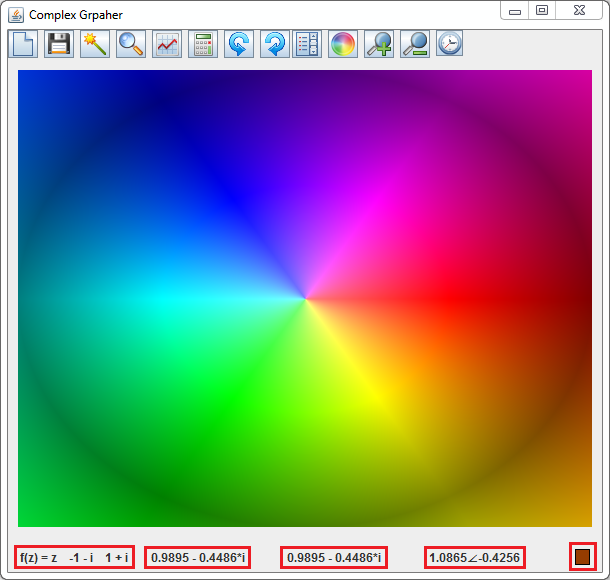
\includegraphics[scale= 0.75]{features}\\
				
				First, from left to right on the toolbar we have
				
				\begin{itemize}
					\item New (
\includegraphics[height=\fontcharht\font`\B]{../src/resources/toolbar/new}) - This will prompt the user to choose the equation, minimum domain and maximum domain, and may then go on to display this new landscape.
					
					\item Save Image (
\includegraphics[height=\fontcharht\font`\B]{../src/resources/toolbar/save}) - Save the landscape as an image file, supported formats include LIST SUPPORTED FORMATS
					
					\item Pan (
\includegraphics[height=\fontcharht\font`\B]{../src/resources/toolbar/pan}) - Pan around the complex landscape, via drag and drop style navigation.
					
					\item Free zoom (
\includegraphics[height=\fontcharht\font`\B]{../src/resources/toolbar/zoom}) - Select a rectangular region of the landscape to zoom in on.
					
					\item Root finder (
\includegraphics[height=\fontcharht\font`\B]{../src/resources/toolbar/newton}) - Finds root using seed value (seed is used as where the user clicks in the landscape) via Newton-Raphson method.
					
					\item Calculator (
\includegraphics[height=\fontcharht\font`\B]{../src/resources/toolbar/calculator}) - Displays a calculator that can be used concurrently with the main application.
					
					\item Undo (
\includegraphics[height=\fontcharht\font`\B]{../src/resources/toolbar/undo}) - Undoes the last action
					
					\item Redo (
\includegraphics[height=\fontcharht\font`\B]{../src/resources/toolbar/redo}) - Redoes the last action
					
					\item Undo/Redo History (
\includegraphics[height=\fontcharht\font`\B]{../src/resources/toolbar/history}) - Display entire undo/history, allowing user to revert to a previous landscape.
					
					\item Centre on Zero (
\includegraphics[height=\fontcharht\font`\B]{../src/resources/toolbar/centre}) - Centres the landscape without changing the magnification.
					
					\item Zoom In (
\includegraphics[height=\fontcharht\font`\B]{../src/resources/toolbar/zoom_in}) - Zooms in about the centre of the landscape
					
					\item Zoom Out (
\includegraphics[height=\fontcharht\font`\B]{../src/resources/toolbar/zoom_out}) - Zooms out about the centre of the landscape
					
					\item Change priority (
\includegraphics[height=\fontcharht\font`\B]{../src/resources/toolbar/speed}) - Toggles between prioritising speed and prioritising accuracy. Prioritises accuracy by default.
				\end{itemize}
			
				Finally, from the left to right red boxes in the status bar, we have
				
				\begin{itemize}
					\item Current landscape - This include the function, $f(z)$ being displayed, and the minimum and maximum domain of the landscape.
					\item Trace input - This represents the value of $z$ at this point in the landscape.
					\item Trace output - This represents the output value, $f(z)$ at this point in the landscape.
					\item Trace polar output - This shows the output $f(z)$ in polar coordinates. The first value being the magnitude, the second being the argument.
					\item Trace colour - The colour of the output value $f(z)$ as per the domain colouring algorithm outlined in \lstinline{complex.Complex.colour()}.
				\end{itemize}
				
			\subsubsection{Equations}
				The complex grapher supports many functions, operators and constants that can be used to display complex landscapes. Supported operators include $+$, $-$, $*$, $/$ and \^{}, which represent addition (binary only) subtraction (and unary negation), multiplication, division, and power, respectively. Supported constants include $e$, $\pi$ and $i$. The following table represents a list of all supported functions. Note that the log function is the only one that takes more than two arguments, all others only take one.
				
				\begin{figure}[H]
					\centering
					\makebox[\linewidth]
					{
						\begin{tabular}{|c|l|}
							\hline 
							\textbf{Function:} & \textbf{Returns:} \\ \hline
							log($z$,$w$) & the logarithm of $z$ to the base $w$ \\ \hline
							neg($z$) & unary negative of $z$, $-z$\\ \hline
							conj($z$) & complex conjugate of $z$\\ \hline
							sqrt($z$) & square root of $z$, faster than $z^{0.5}$\\ \hline
							ln($z$) & natural logarithm of $z$, to the base $e$\\ \hline 
							exp($z$) & constant $e$ raised to the power $z$\\ \hline 
							sinh($z$) & hyperbolic sine of $z$\\ \hline 
							cosh($z$) & hyperbolic cosine of $z$\\ \hline 
							tanh($z$) & hyperbolic tangent of $z$\\ \hline
							sin($z$) & sine of $z$\\ \hline 
							cos($z$) & cosine of $z$\\ \hline
							tan($z$) & tangent of $z$\\ \hline 
							asinh($z$) & inverse hyperbolic sine of $z$\\ \hline 
							acosh($z$) & inverse hyperbolic cosine of $z$\\ \hline 
							atanh($z$) & inverse hyperbolic tangent of $z$\\ \hline
							asin($z$) & inverse sine of $z$\\ \hline 
							acos($z$) & inverse cosine of $z$\\ \hline
							atan($z$) & inverse tangent of $z$\\ \hline 
							inv($z$) & reciprocal of $z$\\ \hline
							mod($z$) & modulus of $z$\\ \hline
							arg($z$) & argument of $z$\\ \hline
						\end{tabular}
					}
					\textit{\caption{Table summarising all supported functions in the Complex Grapher.}}
					\label{table:functions}
				\end{figure}
			
			\subsubsection{Create landscape}
				%%Instruct reader on how to create new landscape, with screenshot of property dialog and how to use it
			
			\subsubsection{Navigate landscape}
				%%Instruct reader on how to navidate through landscape, via pan, free zoom, zoom in, zoom our, centre on zero, and manually selecting the minimum and maximum domain
			
			\subsubsection{Tools}
				Other tools include the root finder (
\includegraphics[height=\fontcharht\font`\B]{../src/resources/toolbar/newton}) and the calculator (
\includegraphics[height=\fontcharht\font`\B]{../src/resources/toolbar/calculator}). The root finder finds the root using the Newton-Raphson method. Selecting a location on the landscape supplies the function with the seed value. After enough iterations, the user is prompted of the final iteration result.
				
				The calculator allows the user to perform calculations independent of the main application. This calculator allows the previous answer to be used in the next calculation, for use in iterative calculations. It also shows the result in a high accuracy, and displays the colour of the result as well.
				
			\subsubsection{Undo/Redo history}
				While changing landscapes (a change in landscape is defined as either a change in equation, minimum domain, or maximum domain.) the grapher stores all previous landscapes. The user can simply undo or redo landscapes as required. 
				
				Alternatively, the user can select the Undo/Redo history button (
\includegraphics[height=\fontcharht\font`\B]{../src/resources/toolbar/history}) and select from the entire history. The history functionality is implemented as the class complex.History, which can be used to implement any type of history.
			
			\subsubsection{Miscellaneous}
				Finally we have the save function (
\includegraphics[height=\fontcharht\font`\B]{../src/resources/toolbar/save}) which allows the user to save the landscape as an image file and the speed priority selector (
\includegraphics[height=\fontcharht\font`\B]{../src/resources/toolbar/calculator}).
				
				The Speed priority selector toggles between creating a landscaper quickly, and creating one accurately. In computer terms this means using fast single precision  or slower, but more accurate double precision values. Note that with a smaller precision, not only is accuracy lost, but values are more likely to underflow or overflow.
		
	\section{How it works}
		%%Give a brief explanation of how it works, followed by a detailed explanation broken up into subsections. Include detailed explanation of coalesced memory, and why various other decisions were made.
		The application parses the formula into a list of tokens, and the minimum and maximum domain into complex constants that the kernel and Java code can use. The list of tokens is stored in RPN format, maximising efficiency and minimising effort during kernel call. The complex grapher application then uses OpenCL (using the Java wrapper JavaCL) to generate the image. First each thread is given its own unique value of $z$, the input value. The is calculated using the minimum and maximum domain, along with the width and height of the complex widget. The kernel then uses a virtual stack for each thread, when each thread activates it evaluates the expression using the postfix evaluation algorithm. Adjacent threads will access adjacent locations in memory during the stack calculations, which allows for coalesced memory access. 
		
		OpenCL is used because it allows for high level parallelism supported by many devices and vendors. It automatically selects the most appropriate device based on a prioritised criteria. The user can prioritise speed (selects the device based on the most the number of compute units) or it can prioritise accuracy (selects fastest device supporting double precision). 
		
		It is worth noting here that choosing double precision does not only allow for the most accurate results, it also allows larger and smaller values to be represented. Functions that increase quickly (such as $z^z$ mentioned earlier) will overflow and underflow faster using single precision. It is highly recommended that the user prioritise accuracy unless the computation is very slow. If the fastest device supports double precision calculations, switching priorities will have no effect on the device. When the application is executed via command line, the application will output the priority type, and which device is used.
		
			\subsection{Complex class}
				The Complex class extends the Commons Math complex class, and adds extra functionality, mostly specific to the Complex Grapher. First it ships with a default constructor, setting the complex value to 0. It adds a \lstinline{color()} function which gets the colour of the complex number as per the domain colouring algorithm. It adds a toPolarString() method, and other trig functions which are not included.
		
			\subsection{Evaluator class}
				The evaluator class is implemented as a functor class. During creation, it uses the \lstinline{setString} method to convert the input equation into a list of tokens stored as member variables. Conversion is performed and validated primarily via static regex strings dynamically built at run time. When the function $f$ is called, it uses the postfix evaluation algorithm on the list of tokens to get $f(z)$. It also exposes the newton-raphson root finder, \lstinline{getStackMax()}, and various other functions used to evaluate the postfix equation. The following listing shows how to use the \lstinline{Evaluator} class:
				
				\begin{lstlisting}[language=Java]
					Use better code listing, with full class, main(args) function users can copy and paste to work without editing
					Evaluator t;
					
					t = new Evaluator("z^2-1");
					
					System.out.println("Result: " + t.f(new Complex()).toString());
				\end{lstlisting}
			
			\subsection{Complex Component widget}
				The complex component serves as a widget to display complex landscapes. It extends the JComponent class, and contains the tools used in the Complex Grapher package encapsulated in a widget. This allows users to import the widget, and use it themselves.
				
				\begin{lstlisting}[language=Java]
					Include listing showcasing Complex Component widget;
				\end{lstlisting}
			
			\subsection{OpenCL Kernel}
				The OpenCL Kernel is responsible for taking the parameters for the landscape and the width and height of the widget, and creating an array if 32-bit coloured pixels (implemented as 32-bit integers). The kernel is also supplied with a large chunk of allocated memory onto which active threads can push and pop items for the postfix evaluation algorithm. The kernel executes in three main steps. 
				
				First the value of $z$ is calculated for the specific thread. It uses linear interpolation in the real and imaginary direction to get the complex coordinate. Secondly, it iterates through all tokens in the token list (passed when the kernel is called) and evaluates them using the postfix evaluation algorithm. Finally, it takes the result of the function $f(z)$ (found at the top of each threads stack) and calculates the colour, passing this to the final results array.
				
				The entire OpenCL code is expressed as three main files, complex.h, real.h and kernel.cl. complex.h contains the bulk of the C code, containing the postfix algorithm, mathematical complex functions and other various functions. real.h Contains various macros for use in complex.h and kernel.cl relating to single and double precision used. kernel.cl contains a single function, the kernel that is called by JavaCL code library. The OpenCL kernel is\\
				
				\lstinputlisting[language=C]{../src/kernel/kernel.cl}
			
			\subsection{User created code}
				The C code used in the OpenCL kernel is linked at runtime. Inside the created .jar file users can locate and edit the files that make up the OpenCL kernel. This allows executable files to be changed to suit the needs of more experienced users. It is important her to distinguish between the Java \lstinline{Evaluator} class and the C OpenCL kernel. Both have separate and distinct (but functionally identical) implementations of the domain colouring algorithm, and other shared functionality. If the user changes the OpenCL kernel, this will result in the landscape changing, but when the user uses the trace colour feature, the results may be different as this is calculated by the \lstinline{Evaluator} class. For both the landscape and Java specific features (trace, calculator, etc.) to match, both Java and C code must be edited.
	
	\section{Limitations}
		As previously mentioned, the Complex Grapher application was created for ease of use, meaning only a small learning curve is required to get started. This means this software does not contain every possible feature associated with complex graphing. That being said, it does contain most of the features users will need when navigating complex landscapes. 
		
		Since the software uses floating point numbers to represent the real and imaginary parts of complex numbers, the complex numbers themselves are subject to the same limitations as floating point numbers. Since the floating point numbers are converted to colours and displayed, (and there are a finite number of colours possible) accuracy of the calculations is not a priority. However, when graphing extremely large or small values, floating precision can overflow or underflow, respectively. This means some regions will show white (NaN or infinite) under single precision where they would still produce values under double precision.
		
		\section{References}
		
			\begin{thebibliography}{100}
				
				\bibitem{mathksu} 
				Math KSU - Complex function grapher,
				\\ \texttt{\href{https://www.math.ksu.edu/~bennett/jomacg/}{https://www.math.ksu.edu/~bennett/jomacg/}}
				
				\bibitem{davidbau} 
				David Bau's Complex Function Viewer,
				\\\texttt{\href{http://davidbau.com/conformal/}{http://davidbau.com/conformal/}}
				
				\bibitem{complexmapper} 
				Complex Mapper 3.6 beta,
				\\\texttt{\href{http://alessandrorosa.altervista.org/pages/downloads.php}{http://alessandrorosa.altervista.org/pages/downloads.php}}
				
			\end{thebibliography}
	
	\section{See Also}
	
		\begin{itemize}
			\item \href{https://en.wikipedia.org/wiki/Domain_coloring}{Domain colouring}
			\item \href{https://en.wikipedia.org/wiki/Reverse_Polish_notation}{RPN notation} (and the postfix evaluation algorithm)
			\item \href{https://devblogs.nvidia.com/how-access-global-memory-efficiently-cuda-c-kernels/}{Coalescing memory}
			\item \href{https://www.khronos.org/opencl/}{OpenCL}
			\item \href{https://github.com/nativelibs4java/JavaCL}{JavaCL}
		\end{itemize}
   
\end{document}







































